\documentclass{article}
\usepackage[utf8]{inputenc}
\usepackage[T1]{fontenc}
\usepackage[catalan]{babel}
\usepackage[vmargin=3cm]{geometry}
\usepackage{lastpage}
\usepackage{lipsum}
\usepackage{graphicx}
\usepackage{parskip}
\usepackage{listings, listings-rust}
\usepackage{hyperref}
\usepackage{url}

\hypersetup{
    colorlinks=true,
    linkcolor=black,
    urlcolor=blue,
    citecolor=red,
}

\graphicspath{ {images/} }

\lstnewenvironment{code}[1][]%
{
   \noindent
   \minipage{\linewidth} 
   \vspace{0.5\baselineskip}
   \lstset{language=Rust, style=colouredRust,#1}}
{\endminipage}

\begin{document}
\begin{titlepage}
	\newcommand{\HRule}{\rule{\linewidth}{0.4mm}} % Defines a new command for horizontal lines, change thickness here
	
	\center

    \vspace*{25px}
    % == Headings ==
	
	\textsc{\LARGE Universitat Autònoma de Barcelona}\\[1.5cm]
	
	\textsc{\Large Treball de Fi de Grau}\\[0.5cm]
	
	\textsc{\Large Informe inicial}\\[0.5cm]
	
	\HRule\\[0.4cm]
	
	{\LARGE\bfseries Disseny i implementació d'un llenguatge de programació amb LLVM}\\[0.4cm]
	
	\HRule\\[1.5cm]
	
	% == Author ==
	
	\begin{minipage}{0.5\textwidth}
		\begin{flushleft}
			\large
			\textit{Autor}\\
			\textsc{Josep Maria Domingo Catafal}
		\end{flushleft}
	\end{minipage}
	~
	\begin{minipage}{0.4\textwidth}
		\begin{flushright}
			\large
			\textit{Tutor}\\
			\textsc{Javier Sánchez Pujadas}
		\end{flushright}
	\end{minipage}
	
	% == Date == 

	\vfill\vfill\vfill % Position the date 3/4 down the remaining page
	
	{\large\today} % Date, change the \today to a set date if you want to be precise

	\vfill % Push the date up 1/4 Of the remaining page
\end{titlepage}

% --------------------------------------
% Table of contents
% --------------------------------------
\tableofcontents
\newpage

% --------------------------------------
% Body
% --------------------------------------
\section{Introducció i el problema a resoldre}
Històricament, generalitzant molt, podem trobar dos tipus de llenguatges: els que 
són ràpids de programar però lents d'executar (ex. Python), i els que són lents 
de programar i ràpids d'executar. En l'última decada han aparegut nous
llenguatges, com ara Go, que intenten situar-se al mig d'aquests dos paradigmes.

\section{Objectiu}
L'objectiu d'aquest treball, és dissenyar i implementar un llenguatge de 
programació que pugui ser executat de forma relativament ràpida, però al mateix 
temps que permeti al programador tenir una expèriencia el més plàcida possible.

Un altre objectiu del llenguatge és intentar minimitzar al màxim els errors que
pot cometre el programador, i per tant reduir el nombre de bugs que es poden
generar en el programa. Per això, serà un llenguatge fortament tipat i inclourà
algunes propietats de llenguatges funcionals com ara la immutabilitat per 
defecte (es pot mutar si el programador vol, però ho ha de fer de forma 
explicita). Si una funció muta l'estat de l'objecte, aquesta ho indicara de 
forma explicita cada cop que es invocada.

Per tal de que el llenguatge permeti un desenvolupament àgil, la gestió de 
memòria serà automàtica.

\section{Definició del llenguatge}

Per importar llibreries externes s'utilitzen imports

\begin{code}
import math
\end{code}

Podem definir constants globals, però no variables
Amb això es busca evitar comportaments estranys del programa i bugs difícils
de trobar, ja que les variables globals poden ser modificada des de qualsevol
lloc.

\begin{code}
const MAX_SPEED = 120;
\end{code}

El punt d'inici del programa és a la funció main.

\begin{code}
fn main() {
    // Les instruccions acaben sempre amb un punt i coma
    println("Hello World!");
}
\end{code}

Per declarar una funció es fa amb la paraula reservada fn, seguit del nom de la 
funció i els paràmetres entre parèntesis, i finalment el tipus del valor de retorn.
Quan l'última expressió no acaba en punt i coma, el resultat serà el que retornarà
la funció. És l'únic cas en que es permet no posar punt i coma.

\begin{code}
fn radius(circumference: i32) i32 {
    circumference / (2 * math.PI)
}
\end{code}

\subsection{Definició de tipus}

Si volem definir tipus genèrics podem definir interficies:

\begin{code}
interface Person {
    fn change_name(name: string) string;
}
\end{code}

Això ens permet tenir diferentes implementacions, amb comportaments diferents.

Per crear tipus propis, és fan servir structs. Permeten definir camps de diferents
tipus i definir metodes que modifiquen l'estat de l'objecte. 

Els camps i els mètodes, per defecte són privats, però es poden fer publics.
En el cas de les funcions amb la paraula reservada "pub". En el cas dels camps,
afegin entre claus (\{\}), les paraules get o set, depenent de si volem que sigui publica
per escriptura, lectura o per les dues coses.

Per implementar una interficie, afegim dos punts i el nom de la interficie just 
després del nom del struct.

\begin{code}
struct User : Person {
    age: i32 { get, set };
    name: string { get };
    id: i32;

    fn change_name(name: string) {
        self.name = name;
    }
}
\end{code}

Amb l'struct anterior, podriem per exemple fer el següent:

\begin{code}
let user = User { age: 24, name: "John Doe" };
user.age = 25;
println(user.name);
\end{code}

Però no podriem modificar el camp \textit{name}.

No es obligatori definir constructor, pero si es vol, l'estandard és crear una
funció estatica que es digui \textit{new}.

\begin{code}
// constructor
pub static fn new(age: i32, name: string) self {
    self {
        age,
        name,
    }
}
\end{code}

Per cridar les funcions estatiques es fa de la següent manera:

\begin{code}
// static: struct_name::static_fn()
let user = User::new(24, "John Doe");
// non-static: object.fn()
user.change_name("Jane Doe");
\end{code}

Podem definir mètodes fora de la definició del struct. Un cas on seria útil,
per exemple, seria quan treballem amb una entitat amb moltes funcions i volem 
dividir-ho en multiples fitxers.

\begin{code}
struct User {
    name: string;
}

pub fn (User) get_name() string {
    self.name
}
\end{code}

Quan un mètode muta l'estat d'un objecte, aquesta funció ho ha d'indicar de forma
explicita. Amb això és busca facilitar la vida al programador a l'hora de programar, 
llegir el codi o debugar, ja que només llegint la crida o la definició, sap que
la funció té efectes secundaris.

Per tal d'indicar aquesta mutació, el programador, ha d'afegir la paraula "mut",
a la definició de la funció, i cada cop que la crida, s'ha d'afegir un signe 
d'exclamació al final de l'identificador (ex: {\ttfamily function!(a, b)}).

El mateix passa amb les variables. Per defecte son immutables. Si es vol mutar 
una variable, s'ha d'afegir la paraula "mut".

\begin{code}
struct User {
    name: string;
    pub mut fn set_name(self, name: string) string {
        self.name = name;
    }
}

fn modify_struct() {
    let mut user = User::new();
    user.set_name!("new name");
}
\end{code}

\subsection{Bucles}

Per tal d'executar repetidament instruccions es fan servir bucles. N'hi ha de 
diferents tipus. El més bàsic es el while:

\begin{code}
let mut a = 0;
let mut i = 0;
while i < 10 {
    a += i;
    i += 1;
}
\end{code}

Un altre opció, és el bucle for:

\begin{code}
let mut a = 0;
// No need for "mut" when declaring i, it's implied
for let i = 0; i < 10; i += 1 {
    a += i;
}
\end{code}

Per iterar arrays, tenim el bucle for in, que recorre l'array element per element.

\begin{code}
let mut a = 0;
for number in numbers {

}
\end{code}


Podem fer break d'un bucle en concret posant una etiqueta:

\begin{code}
// Break outer loop from inner loop
outer: for number in numbers {
    for number in numbers {
        if number % 2 == 0 {
            break outer;
        }
    }
}
\end{code}

O fer un break normal:

\begin{code}
for number in numbers {
    if number % 2 == 0 {
        break;
    }
}
\end{code}

\subsection{Programació Funcional}

Per tal de simplificar algunes operacions que es realitzen amb frequencia, hi 
haurà algunes funcions com ara map, reduce, fold, etc. que ens permetran 
realitzar aquestes operacions amb moltes menys linies. Per tal de poder fer servir
aquestes funcions, és fara ús de "closures".

\begin{code}
fn functional_style(numbers: [i32]) {
    // Functional style with closures
    let numbers_plus_one = numbers.map(|x| -> x + 1);

    let sum = numbers.reduce(|sum, number| -> {
        if number % 2 == 0 {
            sum + number
        }
    });

    if number.any(|x| -> x > 5) {
        print("There's at least one number greater than 5");
    }

    if number.all(|x| -> x > 5) {
        print("All numbers are greater than 5");
    }
}
\end{code}


Les closures, ens permeten tenir funcions de primer ordre, el que vol dir que 
es poden assignar a una variable, per exemple, o ser retornades per una altre 
funció.

\begin{code}
fn two_plus_two() {
    let sum = |a: int, b: int| int -> {
        a + b
    };
    print(sum(2, 2)); // Output: 4
}
\end{code}

Un altre concepte inspirat en llenguatges funcionals, és l'operador pipe (|>). 
Ens permet millorar la lectura de casos tipus el següent:

\begin{code}
validate_age(get_age(parse_data(person)))
\end{code}

Que passaria a ser així:

\begin{code}
let is_valid = 
    person
    |> parse_data
    |> get_age
    |> validate_age;
\end{code}

El que fa el pipe, és passar l'expressió de l'esquerra, com a parametre de la 
funció que hi ha a la dreta.

\subsection{Gestió d'errors}

Les funcions poden returnar el que s'en diu un Result. Un Result, es un enum
que te dos valors possibles: {\ttfamily Ok(T) i Err(E)}, on T és l'element que retorna la 
funció, i E és l'error que retorna la funció.

Al indicar el tipus de retorn com a Result, hem d'indicar el tipus del valor que 
retorna la funció, i el tipus de l'error: {\ttfamily Result<TipusOk, TipusErr> }

\begin{code}
fn divide(a i32, b i32) Result<i32, string> {
    if b == 0 {
        return Err("Divide by zero");
    }
    return Ok(a / b)
}
\end{code}

Quan cridem a la funció, hem de comprovar que no ens hagi retornat cap error:

\begin{code}
fn call_divide() -> Result<i32, string> {
    let result = match divide(5, 0) {
        Ok(num) => num,
        Err(err) => return Err(err),
    }

    print("The result is: ", result);
    Ok(result)
}
\end{code}

Com que pot ser una mica engorros haver de comprovar l'error en cada crida, hi
ha l'operador "?" que ens permet retornar imediatament en cas que el resultat
sigui un error:

\begin{code}
fn call_divide() -> Result<i32, string> {
    let result = divide(5, 0)?;
    print("The result is: ", result);
    Ok(result)
}
\end{code}

D'aquesta manera, com que la funció divide ens retorna un error, call\_divide,
retorna immediatament l'error i ja no s'executa el print. En cas que divide hagués
retornat un Ok, l'execució hagués continuat. Cal destacar que la funció que 
fa servir l'operador "?", també ha de retornar un Result, ja que implica que pot
retornar un error.

\subsection{Referències}

Si a un tipus l'hi afegim un {\ttfamily \&} a davant, passara a ser una referència. Les 
referències en permeten apuntar directament a una posició de memòria, i passar
aquest apuntador, sense la necessitat de copiar l'objecte. Per defecte les
referències, igual que les variables, són immutables, però es poden mutar, si 
afegim la paraula mut. En cas de que la referencia sigui mutable, es modificara
la posició de memoria a on apunta, per tant totes les referencies que llegueixin
d'aquesta posició de memoria veuran el canvi.

\begin{code}
// References are immutable by default but we can make them mutable
fn references(numbers: &[i32], other_numbers: &mut [i32]) {
    for number in numbers {
        print(number);
    }

    for number in other_numbers {
        *number += 1; // This will modify the original vector
    }
}
\end{code}

\section{Passos a seguir}

Abans de començar a fer qualsevol cosa, em d'escollir la tecnologia amb la que
volem implementar el compilardor. Per aquest projecte, s'ha escollit a Rust com
llenguatge de programació i a LLVM \cite{llvm_website} com a toolchain per a la generació de codi
del back-end. LLVM ens permetra generar assemblador per pràcticament qualsevol
arquitectura que existeixi avui en dia, sense haver de fer cap esforç adicional.
Només en haurem d'encarregar de generar la IR de LLVM, i aquest s'encarragara de
generar l'assemblador a partir del IR. La API de LLVM esta només per C/C++, per
tant també farem servir una llibreria que es diu Inkwell \cite{inkwell}, que ens ofereix una
API per a Rust, interectuant amb la API de C.

Un cop escollides les tecnologies el següent pas es crear un entorn i una 
estructura de projecte base, on hi podem anar afegint totes les funcionalitats
adicionals.

Per tal d'implementar les funcionalitats definides, seguirem un procés similar
amb totes. Haurem de fer tres coses:

\begin{enumerate}
    \item \textbf{Lexer}: El lexer s'encarrega de llegir el nostre codi, i 
        convertir-lo a un seguit de tokens. Un token és un conjunt de caracter 
        en el codi font que te algun signidicat en el lleguatge, com ara una paraula 
        clau del lleguatge (if, for, ...), o l'identificador d'una variable.
        Per cada funcionalitat, haurem d'adaptar el Lexer perque ens reconegui 
        aquests nous token que s'introdueixin al llenguatge.
    \item \textbf{Parser}: El parser recorre la seqüència de tokens que ens
        retorna el lexer i l'hi busca el significat. El resultat del parser és
        un arbre sintàctic, que ens indicarà com s'han d'executar les instruccions.
        Per cada nova funcionalitat, haurem de modificar el parser perquè pugui
        interpretar els nous constructes.
    \item \textbf{Generació de codi}:
\end{enumerate}


\section{Metodologia i planificació}
Per tal d'organitzar el desenvolupament del projecte s'ha optat per una metodologia
basada en sprints, on cada sprint té un duració d'una setmana. Donat que és un 
projecte gran, s'ha dividit en un conjunt d'epiques, que representen un conjunt 
de funcionalitats. Cada una d'aquestes epiques, conte un seguit de subtasques, i
completar cada una d'aquestes epiques requereix d'uns quants sprints. Les epiques
que s'han definit són les següents:

\begin{enumerate}
    \item \textbf{Implementació mínima de l'especificació}\\
        Implementar tota la funcionalitat basica per poder fer programes senzills.
        Inclou operacions aritmetiques, funcions, control de flux bàsic (if 
        statements i bucles while) i declaració de variables.

    \item \textbf{Declaració de tipus} \\
        Implementar la funcionalitat necesaria per definir tipus de dades 
        propis (structs, interficies i type aliases).

    \item \textbf{Collections}\\
        Implementació d'arrays estàtics, arrays dinàmics i tuples.
    
    \item \textbf{Mecanisme de gestió d'errors}\\
        Implementar un mecanisme per tal de gestionar errors en temps d'execució.
    
    \item \textbf{Syntactic sugar}\\
        Implementació de "Syntactic sugar", per tal de simplificar operacions 
        que s'utilitzen frequentment. Inclou bucles for in, match (similar a un
        switch), list comprehension, etc.
    
    \item \textbf{Support for functional style programming}\\
        Afegir suport per programació d'estil funcional, integrant funcions com 
        ara map, reduce, fold, etc.
\end{enumerate}

Per tal de gestionar totes aquestes epiques, les seves subtasques i els sprints,
es fara servir Jira, un programa de gestió de projectes que ho facilita molt.

\begin{figure}
    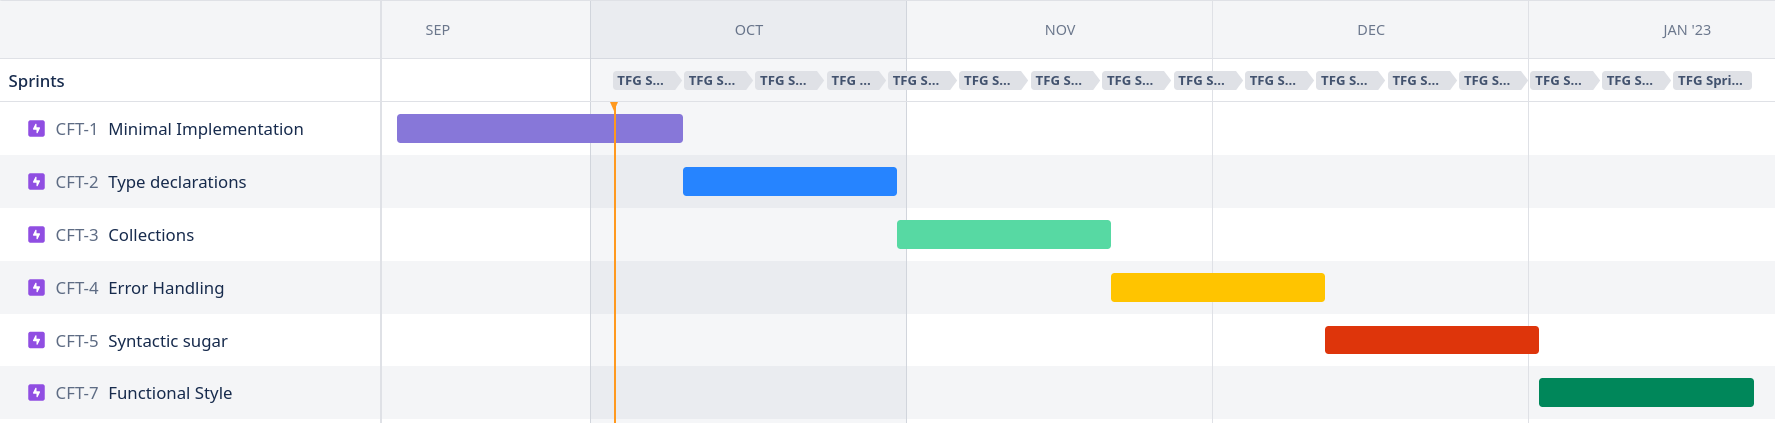
\includegraphics[width=\linewidth]{roadmap}
    \caption{Roadmap on es mostren les diferents èpiques i l'espai de temps on s'han de desenvolupar}
\end{figure}

Cada una d'aquestes funcionalitats, generalment, es divideixen en tres 
subtasques principals: implementar el lexer, implementar el parser i 
implementar la generació de codi.

\section{Inspiració}
La gran majoria de funcionalitats descrites en l'apartat anterior han siguit 
inspirades d'altres llenguatges ja existents. La sintaxi és similar a la de Rust,
però agafant conceptes d'altres llenguatges i paradigmes. Per exemple:

\begin{enumerate}
    \item \textbf{List comprehension}: Python
    \item \textbf{Iteradors (map, reduce, ...)}: Llenguatges funcionals, Javascript, Rust, C\#...
    \item \textbf{Result i Option}: Rust, Scala, Swift
    \item \textbf{Immutabilitat}: Llenguatges funcionals, Rust, Swift
    \item \textbf{Structs}: C, Go, Rust
    \item \textbf{Pipes}: Elixir, F\#
    \item \textbf{Referències}: C++, Rust, Go
    \item \textbf{Sintaxi get, set}: C\#
    \item \textbf{Expression-oriented}: Scala, Rust, Kotlin
\end{enumerate}

\begin{thebibliography}{9}
\bibitem{llvm_website} 
The LLVM Compiler Infrastructure, \url{https://llvm.org}

\bibitem{inkwell} Inkwell, \url{https://github.com/TheDan64/inkwell}

\bibitem{llvm_kaleidoscope} LLVM Kaleidoscope Tutorial: Implementing a Language with LLVM,\\ \url{https://llvm.org/docs/tutorial}

\bibitem{crafting-interpreters}Crafting Interpreters, Bob Nystrom, \url{http://www.craftinginterpreters.com}

\end{thebibliography}
\end{document}
